\section{An Example}\label{sec:case}
We use the x86 code snippet shown in Figure~\ref{fig:examplecode} as an example to illustrate how \DSVMP operates.
``\texttt{STARTSDK}" and ``\texttt{ENDSDK}" are used to mark the begin and end of the code region respectively,
and ``00401036" and ``00401038" are the address the two assembly instructions.

\begin{figure}[t!]
\scriptsize
\begin{lstlisting}
STARTSDK
00401036 mov eax, ebx
00401038 sub eax, 03
ENDSDK
\end{lstlisting}
%\vspace{-2mm}
\caption{Example assembly code snippet for a code region to be protected.}
%\vspace{-4mm}
\label{fig:examplecode}
\end{figure}

\subsection{Process of protection}
Firstly, \DSVMP extracts the critical code from the target program that disassembled into native instruction, here will automatically insert two additional instructions (``\texttt{push 0x40103b}" and ``\texttt{ret}") after two key
instructions in order to jump back to execute the native code
after the protected code region, as showed in figure~\ref{fig:examplecode}.
It then converts the native instructions to virtual instructions according to a translation convention.
The resulted virtual instructions is given in Table~\ref{tab:Tab.1}.
\DSVMP's bytecode instructions are based on a stack machine model.
Here the \texttt{load} instruction is used to push operands into the stack,
and the \texttt{store} instruction is used to pop results out from the stack
and store the result to the virtual context (VMContext).

\begin{table}[!h]
\scriptsize
\begin{center}
\caption{Generated virtual instructions for the example shown in Figure~\ref{fig:examplecode}\label{tab:Tab.1}}
{\tabcolsep6pt\begin{tabular}{@{}cllll@{}}
  \hline
    & \textbf{Instr.1} & \textbf{Instr.2} & \textbf{Instr.3} & \textbf{Instr.4} \\
  \hline
  \textbf{ NI} & \texttt{mov eax, ebx} & \texttt{sub eax, 0x03} & \texttt{push 0x40103b} & \texttt{ret} \\
  \hline
  \textbf{ VI} & \tabincell{l}{\texttt{move 0x08}\\\texttt{load}\\\texttt{move 0x04}\\\texttt{store}} & \tabincell{l}{\texttt{move 0x04}\\ \texttt{load}\\ \texttt{load 0x03}\\ \texttt{sub}\\ \texttt{store}\\ \texttt{move 0x04}\\ \texttt{store}} & \texttt{load 0x40103b} & \texttt{ret} \\
  \hline
\end{tabular}}{}
\end{center}
\vspace{-2mm}
Notes: In the table, ``NI" indicates the native x86 instructions, and ``VI" donates the virtual instructions.
Here, our system inserts ``Instr.3" and ``Instr.4" in order to jump back to execute the native code after returning from the protected code region.
\end{table}

After translating the native code to virtual instructions, we use the deformation engine to transform the initial bytecode handlers set. For this example, our system with 2 VMs configurations, so we generate two sets of bytecode handlers which are semantically equivalent but are implemented in different ways.
Then we randomly shuffle the serial numbers of these handlers, resulting in two new sets of handlers: \texttt{HAS1} and \texttt{HAS2}.  Each set of bytecode handlers is associated with two bytecode instruction sets: \emph{DriverDataSet11} and \emph{DriverDataSet12} for \texttt{HSA1} and \emph{DriverDataSet21} and \emph{DriverDataSet22} for \texttt{HSA2}. The resulted program is illustrated in Figure~\ref{fig:Fig.ex}. We store the virtual instructions in the bytecode format,
and will fill the critical code segment to be protected with junk instructions.

Finally, \DSVMP create a new code section attached to the end of the target program.
The new code section contains the implementation of the handlers, different sets of bytecode instructions,
dispatchers and other VM components such \texttt{VMContext} and routines such as
\texttt{VMInit} (used to initialize the VM) and \texttt{VMExit} (use for cleanup before exiting the VM).



\subsection{Runtime execution}
Runtime execution of the protected code region is illustrated in Figure \ref{fig:Fig.ex}, which follows a number of steps:
\begin{itemize}
\item \textbf{Step1:} The entry of the protected code segment contains an ``\texttt{jmp VMInit}" instruction. This transfers the control to the VM initialization routine, \texttt{VMInit}, which saves the native host context and initializes the virtual context.
\item \textbf{Step2:} Next, a dispatcher starts working. It randomly selects a VM, we assume that \texttt{VM2} is chosen at beginning, and then it fetches a bytecode from the \emph{DriverDataSet21}. After decoding, the dispatcher gets a bytecode ``\texttt{6a}". It then jumps to execute ``\texttt{0x6aHandler}", and the next bytecode ``\texttt{07}" is its operand.
\item \textbf{Step3:} A control unit execute (see Section~\ref{sec:mb}) before exiting the ``\texttt{0x6aHandler}". The control unit randomly selects to execute another handler, ``\texttt{0x85Handler}", or return the controller to the dispatcher. If it chooses to return to the dispatcher, the program execution moves to Step 5.
\item \textbf{Step4:} Assume that the control unit decides to direct execute the next handler, ``\texttt{0x85Handler}". It will then fetch a bytecode from \emph{DriverDataSet22}, decoding it and getting the offset address of ``\texttt{0x85Handler}" . Using the offset, the control unit will jump to execute ``\texttt{0x85Handler}". After executing the handler, the program execution moves to Step 3.
\item \textbf{Step5:} If the control unit chooses to return the controller to a dispatcher, it will randomly select a dispatcher to continue the execution. Then, the program moves to Step 6.
\item \textbf{Step6:} The selected dispatcher randomly selects one VM to use. The dispatcher fetches a bytecode from this VM, decoding the bytecode to get the handler serial number.
    It then jumps to execute the handler. After executing the handler, the program execution moves to Step 3.
\item \textbf{Step7:} Step 3 and Step 4 are iterated until all the bytecodes get executed. The finally step is to invoke the \texttt{VMExit} to restore the native context and to continue executing the rest of target program.
\end{itemize}

\begin{figure}[!t]
  \centering
  % Requires \usepackage{graphicx}
  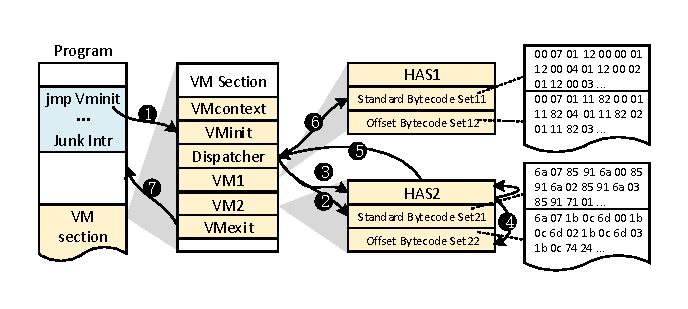
\includegraphics[width=0.7\columnwidth]{figure/figex.pdf}\\
  \caption{The execution process of the protected program. Here each VM has two sets of bytecode instructions and one set of handlers.}\label{fig:Fig.ex}
  %\vspace{-5mm}
\end{figure}